\chapter{Functionality}
\label{chapter:functionality}

ACE is a platform independent collaborative text editor. It features basic text editing as well as collaborative editing functionality.

\begin{figure}[H]
\begin{center}
  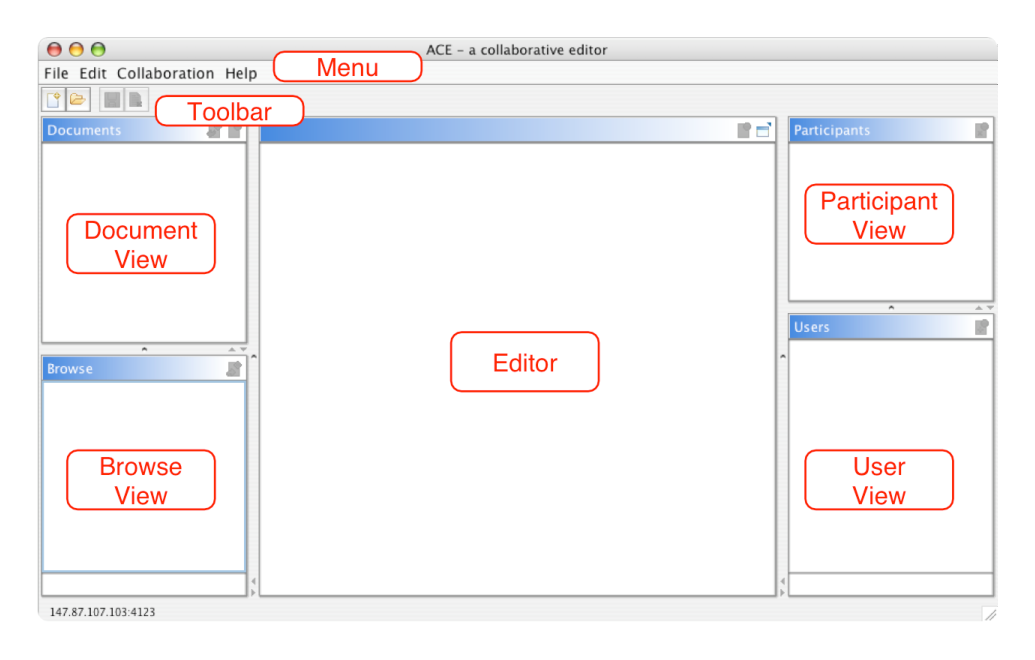
\includegraphics[height=3.1in, width=5.1in]{../images/finalreport/application_ace_overview.eps}
\caption{ACE Overview}
\end{center}
\end{figure}

ACE allows to \emph{create new}, \emph{load} and \emph{save} documents. Further, it allows to have multiple open documents at the same time and to switch between them. Additionally, the familiar cut/copy/paste actions are implemented. See section \ref{sect:algorithm.undoredo} for a justification why the ACE editor does not support undo/redo.

All users running ACE are automatically discovered on the same local area network (LAN). Further, it is possible to explicitely discover users that are not on the same LAN. All discovered users are displayed in the graphical user interface of ACE.

A user can \emph{share} his documents by \emph{publishing} them. A published document is discovered automatically by all other users running ACE. Every user has a list of documents that have been published by other users. The publisher can \emph{conceal} a published document so that collaborative editing is no longer possible.

A document shared by another user can be \emph{joined}. To join a document the user sends a join request to the \emph{publisher}. The publisher either accepts or rejects a join request (a simple yet effective \emph{access control}). If the join request is accepted, the joining user becomes a \emph{participant} in the editing \emph{session}. He can start participating by editing the shared text document independently. A user that no longer wants to participate \emph{leaves} the session.

The publisher of a document can \emph{invite} other users to join a session. An invitation can be accepted or rejected by the invited user. Misbehaving participants can be \emph{kicked} from the session by the publisher. A kicked user is added to the session's blacklist which prevents that the user can rejoin the session.

In an editing session different participants session are distinguished by use of colors. The text background edited by a particular participant is colored in that user's color. Additionally, the current cursor position and selection of other participants is also displayed. This so-called \emph{awareness information} helps to avoid unecessary editing conflicts, for instance when two participants try to edit text at the same location.

ACE has an intuitive user interface. Different views represent the current application state, including a list of open documents, the currently discovered users, shared documents, and participants of each editing session. The views can be minimized to show as much as possible of the currently edited document. Further, the application features a simple preferences system, which allows to set the nick name of the local user and to change the font size used by the text editor.

\begin{figure}[H]
\begin{center}
  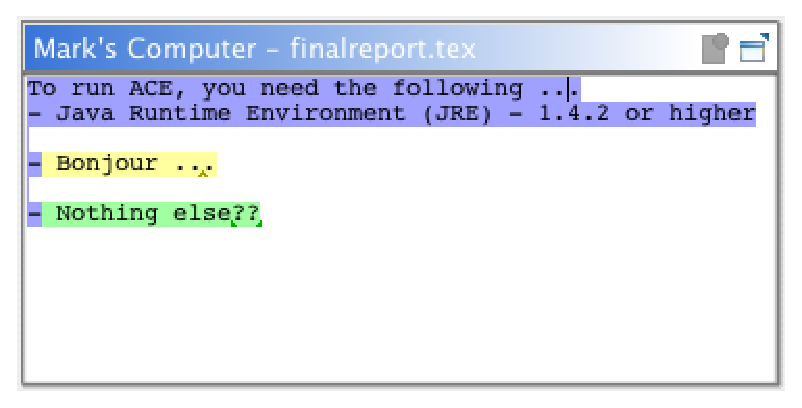
\includegraphics[height=2.5in, width=5.12in]{../images/usermanual/editor_collab_3users.eps}
\caption{Three Users writing in one Document}
\end{center}
\end{figure}

The functionality fulfills the mandatory goals and some optional goals set at the beginning of the semester project as described by the \emph{System Requirements} document. A description of the work done before the diploma project can be found in overview section \ref{sect:overview.previouswork}.
